\section{Methodology} % 3 Pages  
\label{sec:method}


\subsection{Design Overview}
\label{sec:overview}


% %\vspace{-2pt}


We propose STOF, accelerating Sparse Transformer inference with flexible masking patterns and operator fusion schemes on GPU.
%As shown in Figure~\ref{fig:4-method-overview}, 
STOF consists of a \textit{unified MHA module} and an \textit{operator fusion module}. The unified MHA module integrates row-wise and block-wise kernels with different storage formats, each with unique optimizations. The operator fusion module is embodied as the interaction between the fusion scheme converter and the hierarchical search engine. 

Figure~\ref{fig:4-method-overview} illustrates the design overview of STOF. STOF divides the sparse Transformer model into MHA structure and downstream operators. This ensures both the customization of MHA and the flexibility of operator fusion. For MHA structure, STOF maps its calculations directly to GPU kernels with fine-grained optimization. The kernel selector determines the MHA kernel by applying an analytical model that takes hardware specifications into account. For downstream operators, the scheme converter expresses the fusion scheme as a binary array through hash coding upwards and maps it to compilation templates through numerical decoding downwards. The search engine initializes scheme, expands fusion, and samples parameters via analytical modeling, performance feedback, and reward algorithm, respectively.


\begin{figure}[htbp]
  \centering
  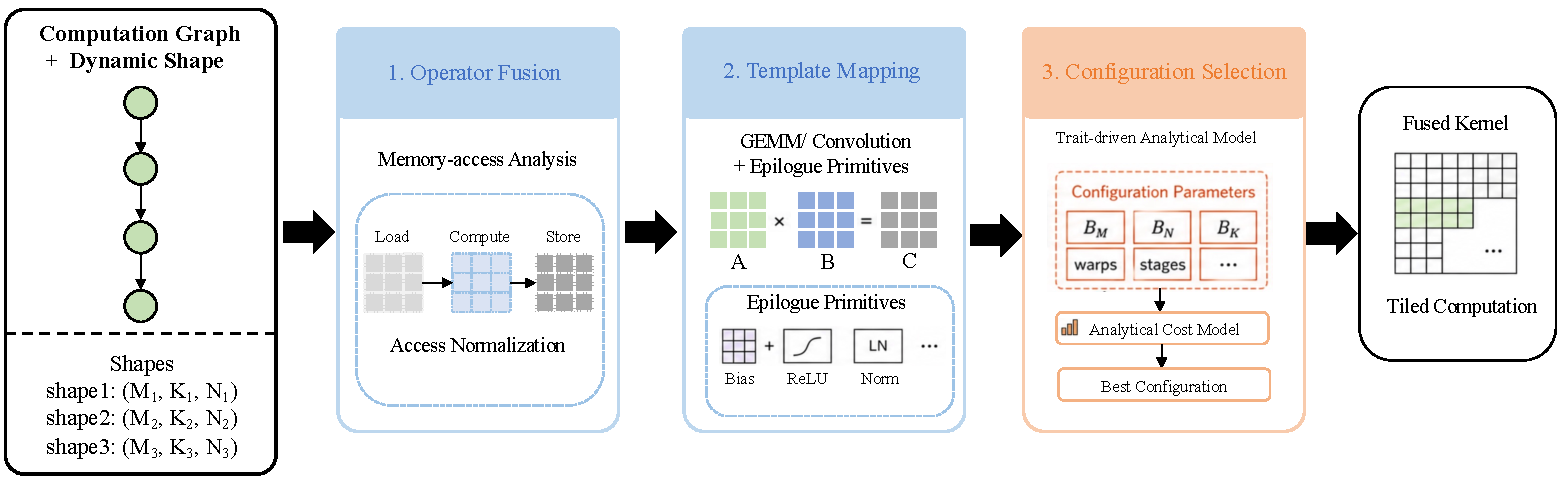
\includegraphics[width=\linewidth]{figures/4-method-overview.pdf}
  % 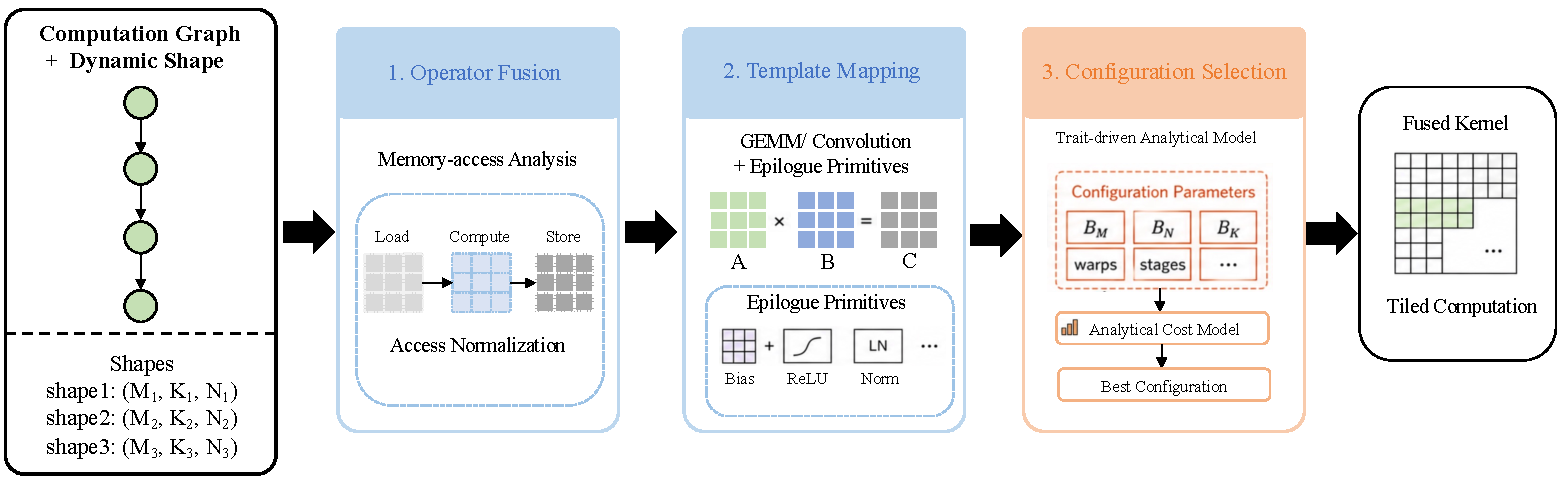
\includegraphics[scale=0.44]{figures/4-method-overview.pdf}
  %\vspace{-8pt}
  \caption{The design overview of STOF.}
  \label{fig:4-method-overview}
\end{figure}



We have implemented two sets of kernels depending on the data partitioning granularity. The row-wise kernel slices $Q$ into rows to achieve high locality. Moreover, the row-wise kernel applies shuffle within a warp and eliminates the synchronization among warps, improving performance at small input sizes. In contrast, the block-wise kernel is more general with fine-grained block partitioning, where $Q$, $K$, and $V$ are partitioned into sub-blocks and put into SMEM to utilize the GPU memory hierarchy. Since row partitioning can be regarded as an extreme case of block partitioning, we elaborate on the block-wise optimizations in Section~\ref{subsec:unified-mha}.

% shepherd 补充内容：
% 1）Description of fusion and pseudocode
% 2）Implementation in general fashion
% 3) Concerns about generality
The main takeaway of STOF is a novel co-design that bridges manual kernel implementation for sparse MHA structure and automatic fusion for dense downstream operators. Specifically, the sparsity in STOF is exclusively handled within the MHA module, where mask-based computation is explicitly managed by customized kernels.
% (with pseudocode provided in Algorithm~\ref{alg:AttnKernel})
All subsequent operators after MHA are dense and executed via template-based fusion, ensuring both high performance and compositional flexibility. Beyond the specific optimizations for Transformer architectures, the core methodology of STOF is readily extensible to emerging LLM architectures. For instance, in Mixture-of-Experts (MoE) models~\cite{cai2025survey}, we can accelerate activated experts via specialized kernels while optimizing the routing logic through template-based fusion, potentially supporting dynamic computation paths at minimal cost.

%Beyond the specific optimizations for Transformer architectures, the core methodology of STOF, including hand-tuned kernels and the template-based fusion approach, is readily extensible to emerging LLM architectures. For instance, in Mixture-of-Experts (MoE) models, STOF can accelerate activated experts via specialized kernels while optimizing the routing logic through template-based fusion, thus supporting dynamic computation paths without sacrificing end-to-end efficiency. The main takeaway is a novel co-design that bridges manual kernel implementation for sparse MHA and automatic fusion for dense downstream operators. In a broader context, STOF can serve as an efficient inference backend, offering hand-optimized kernels for critical sparse operations and a lightweight, template-based fusion engine for surrounding dense operators.



\subsection{Unified MHA Kernels}
\label{subsec:unified-mha}
% 第2段：描述 block-wise 的 BSR 结构
\subsubsection{Sparse Storage Format}

Figure~\ref{fig:4-method-Attn-kernel} shows the block-wise computation with a sparse storage format that can represent arbitrary mask. Inspired by literature~\cite{niu2022tilespgemm, fan2025spinfer}, we adopt a two-level storage format combining Block Compressed Sparse Row (BSR) and bitmap, preserving sparsity while enabling structured computation. As shown in Figure~\ref{fig:4-method-Attn-kernel}, we abstract two levels as OuterTile (OT) and InnerTile (IT) to reveal globally skipped blocks and intra-block element distribution, respectively. Each OT is composed of 64 8$\times$8 ITs (only 4 are shown in the figure for clarity). An OT is marked as ``full'' if all of its ITs are not empty, otherwise ``part''. For the ``full'' OTs, the difference between $full\_row\_ptr[i]$ and $full\_row\_ptr[i - 1]$ indicates the number of ``full'' OTs in the $i$-th row. The array $full\_col\_idx$ specifies the column indices of ``full'' OTs. For example, as can be inferred from $full\_row\_ptr$ and $full\_col\_idx$ arrays in the figure, the column indices of ``full'' OTs in the $2$-nd row are 0 and 2.

 %the length of the array $full\_row\_ptr$ is $\lceil\frac{seq\_len}{OT\_Size\_M}\rceil + 1$, \textcolor{red}{where $OT\_Size\_M$ is XXX}. 

%use \textit Outer Tile(OT) to represent globally skipped blocks at the first level and \textit{InnerTile(IT)} to encode fine-grained mask patterns at the detail level. \textit{OuterTiles} are classified into ``full'' and ``part'' according to the internal element distribution, where the classic size is $64\times64$. For the ``full'' blocks, the length of the array $full\_row\_ptr$ is $\lceil\frac{seq\_len}{OT\_Size\_M}\rceil + 1$. The difference between $full\_row\_ptr[i]$ and $full\_row\_ptr[i - 1]$ indicates the number of ``full'' blocks in the $i$-th row. The array $full\_col\_idx$ specifies the column indices of ``full'' blocks. As seen, the column indices of ``full'' blocks in the $2$-nd row are 0 and 2.

%To the best of our knowledge, this is the first time this combination is used to express masks in sparse Transformer,

% 第3段：描述 bitmap 的存储机制 --- 大图右边
For the  ``part'' OTs, there are also two similar arrays including $part\_row\_ptr$ and $part\_col\_idx$. The $part\_col\_idx$ further points to the corresponding IT with sparse element distribution.
%However, the $part\_col\_idx$further points to the corresponding \textit{InnerTile}, which stores the finest-grained mask information. Internally, each ``part''-type \textit{OuterTile} is composed of 64 \textit{InnerTiles}, each of size $8\times8$ (only four are illustrated in Figure~\ref{fig:4-method-Attn-kernel} for clarity). 
Since each IT contains exactly 64 elements, it can be efficiently represented by a single \texttt{uint64} value. 
Consequently, for each ``part'' OT, the internal mask information is stored as a \texttt{bitmap\_mask} array consisting of 64 \texttt{uint64} elements.
During the processing of the innermost loop, each \texttt{bitmap\_mask[i]} is retrieved to obtain the precise masking pattern. By combining the structures of ``full'' and ``part'' OTs, we obtain $load\_row\_ptr$ and $load\_col\_idx$ arrays that directly specify the location of non-empty OTs in the mask.

%During the processing of the innermost mask, the corresponding \texttt{bitmap\_mask[i]} is retrieved and decoded to obtain the precise mask pattern. By combining the data structures of the ``full'' blocks and ``part'' blocks, we obtain $load\_row\_ptr$ and $load\_col\_idx$ arrays that directly represent the number of blocks and column indices containing non-zero elements per row in the mask.



\label{sec:fmk}
% SQX: 还是太占空间了，或者想办法变为单栏，或者就压扁
\begin{figure}[htbp]
  \centering
  % 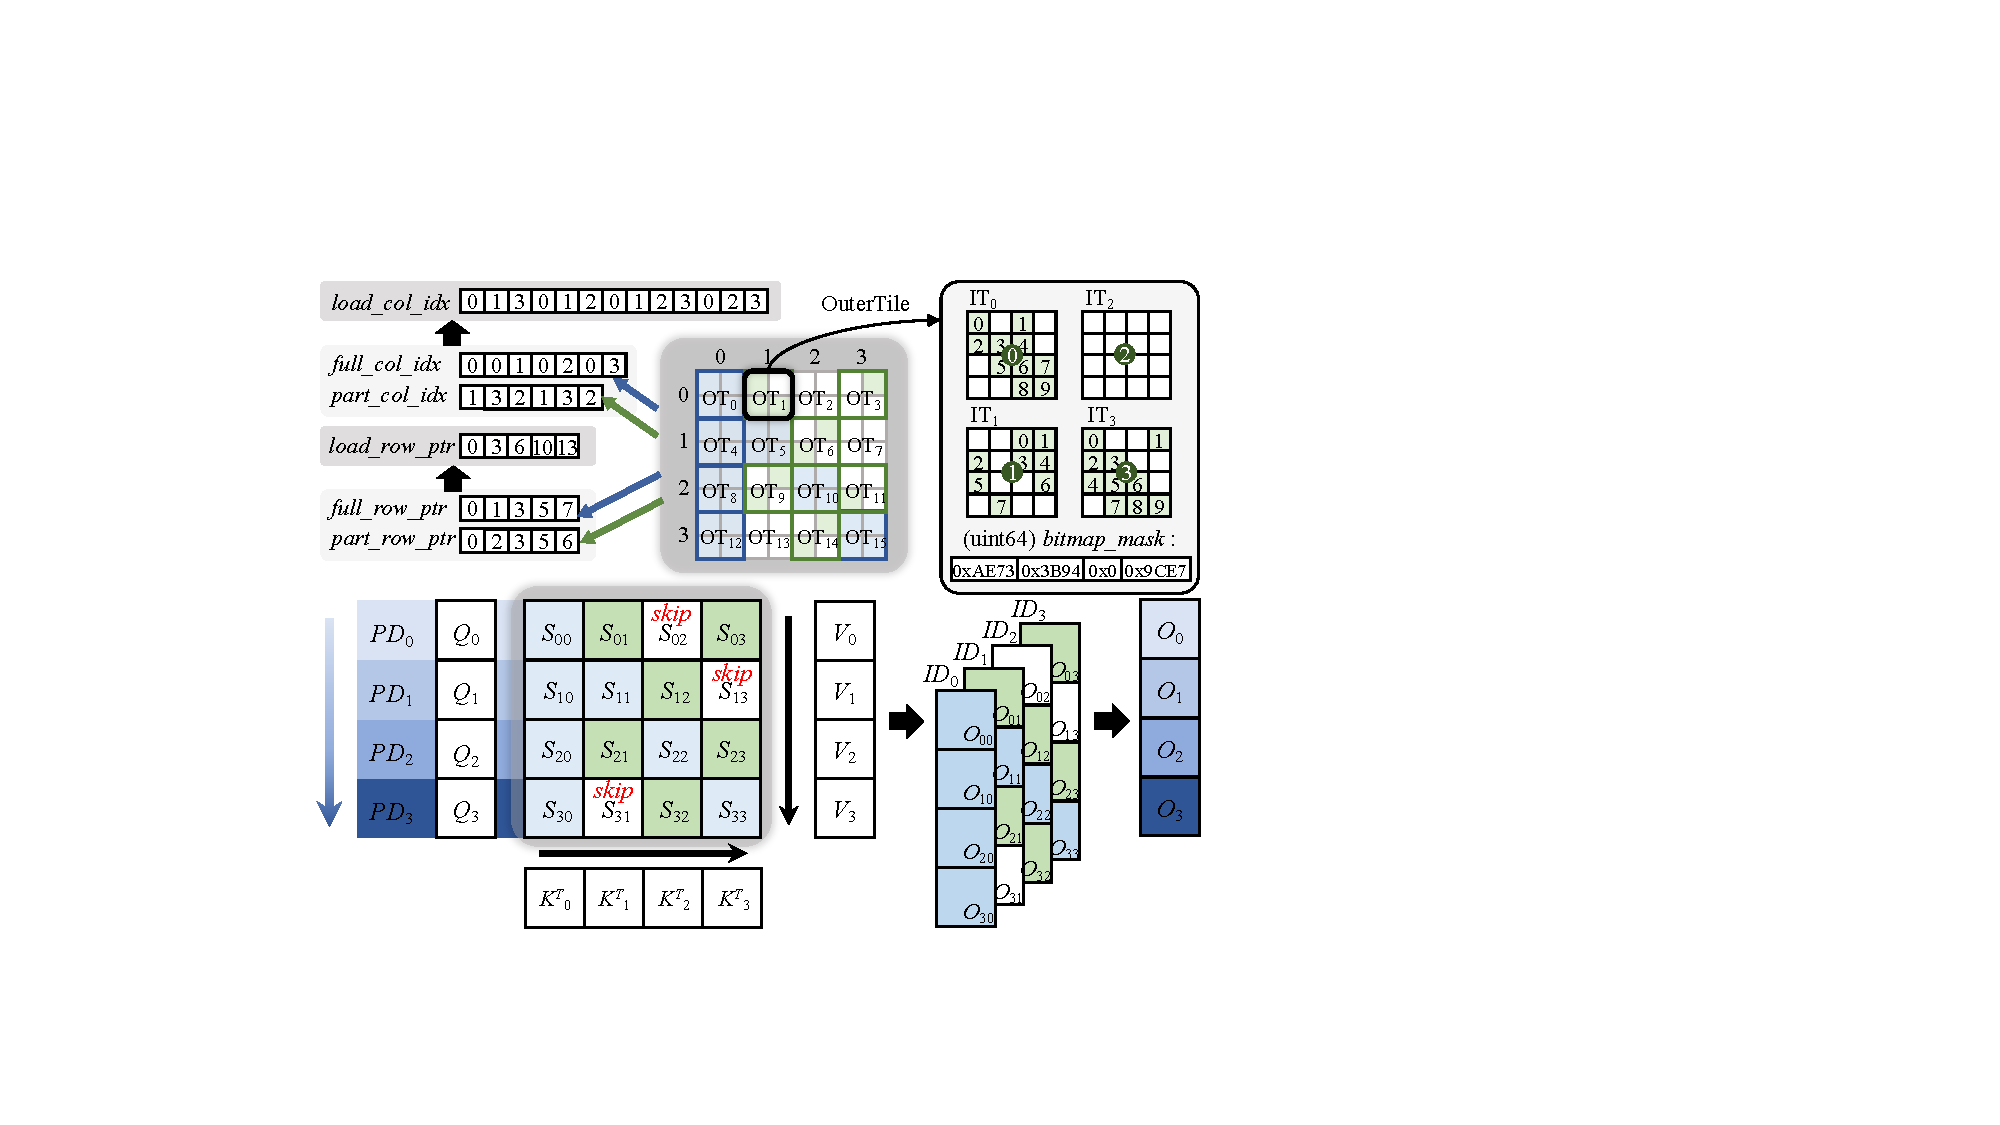
\includegraphics[scale=0.46]{figures/4-method-Attnkernel.pdf}
  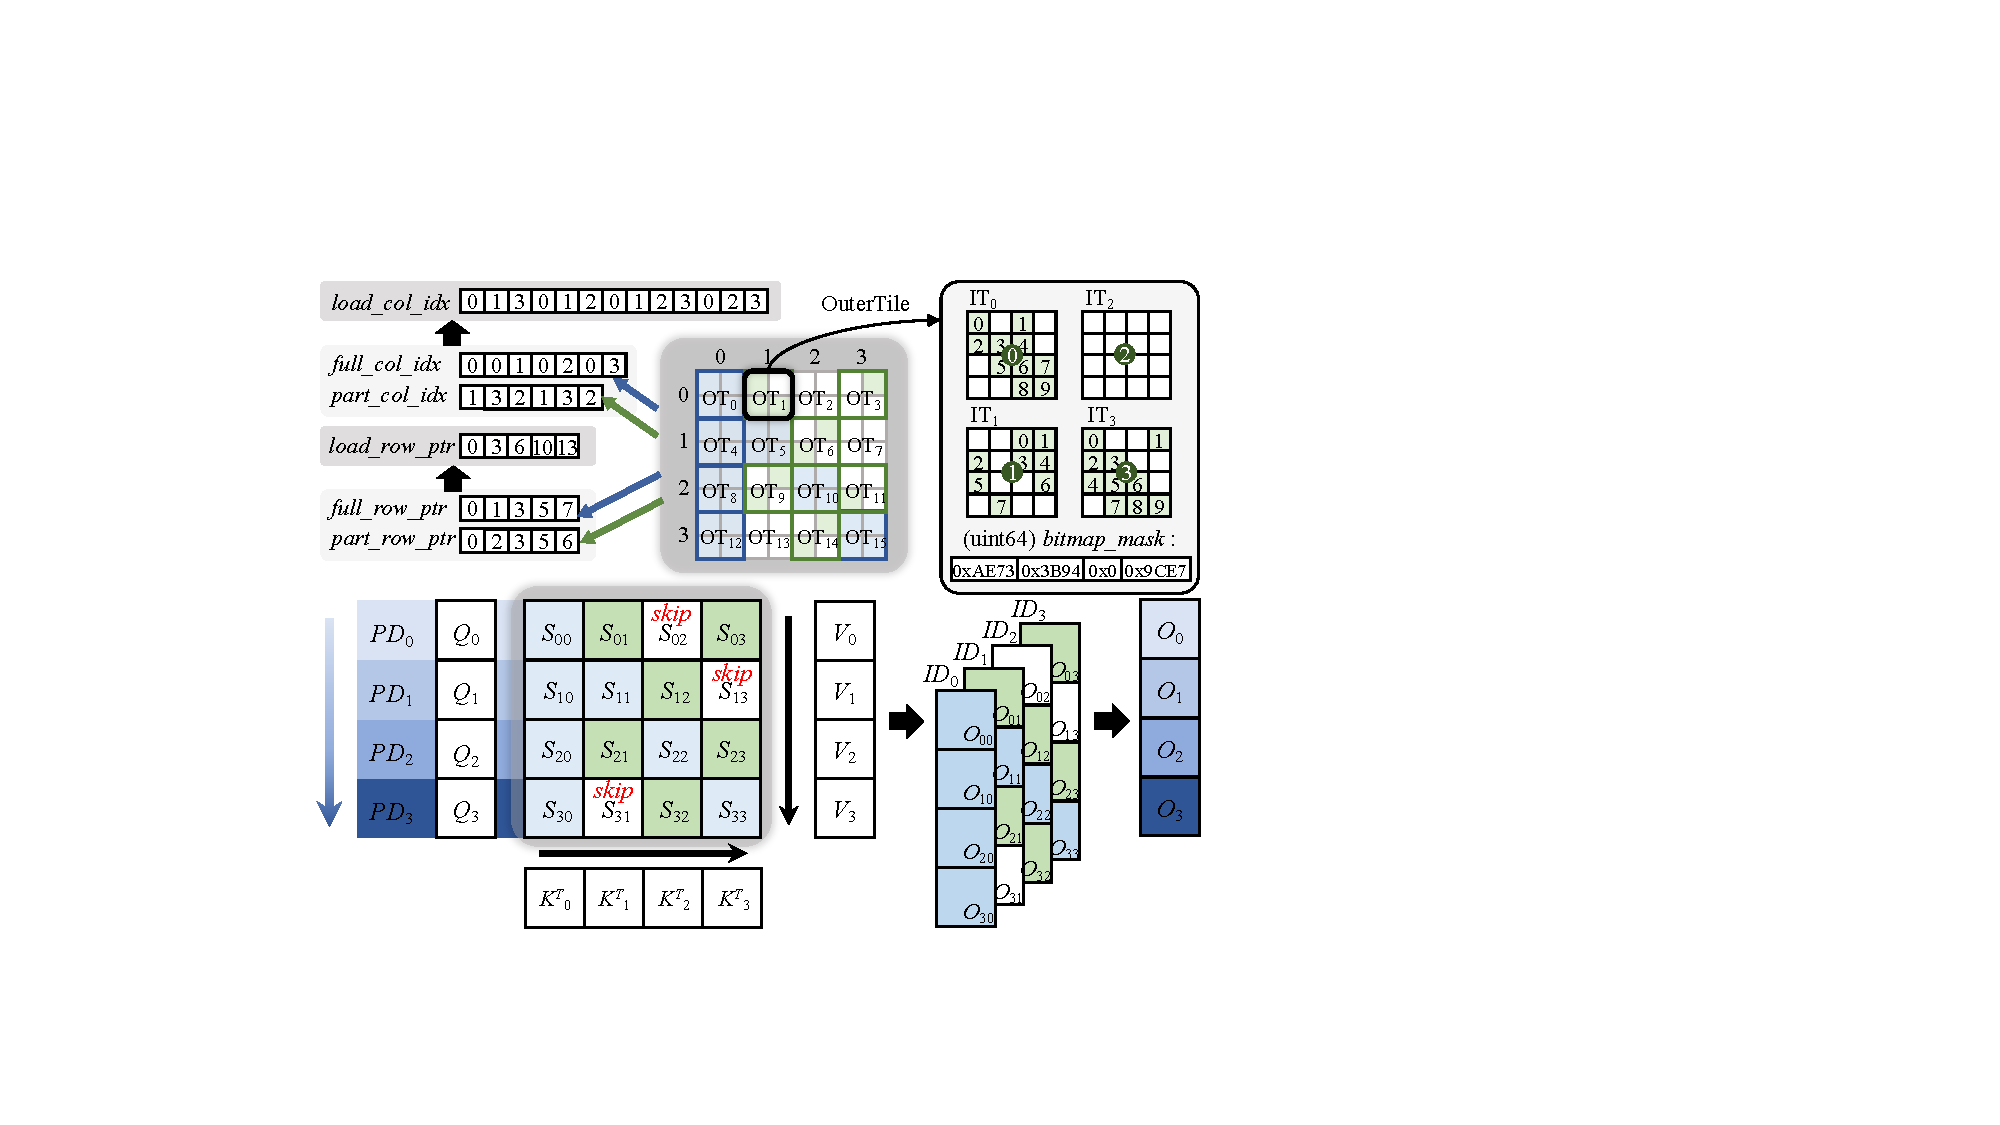
\includegraphics[width=\linewidth]{figures/4-method-Attnkernel.pdf}
  %\vspace{-5pt}
  \caption{MHA computation with two-level storage format.}
  \label{fig:4-method-Attn-kernel}
\end{figure}
% %\vspace{-5pt}



% 第4段：描述跳过的设置，编程分块思路， 主要是介绍伪代码
\subsubsection{Kernel Implementation}
%In consistent with previous works~\cite{wang2024flashmask, dong2024flex, dao2023flashattention2}, 
We cut the input tensor $Q$ into sub-blocks of size (\textit{OT\_Size\_M}, \textit{head\_size}) along the $seq\_len$ dimension, as illustrated in Algorithm~\ref{alg:AttnKernel}.
Each sub-block $Q_i$ (line 2) corresponds to a Row-\underline{P}arallel \underline{D}imension ($PD_i$), where $i \in [0,\lceil\frac{seq\_len}{OT\_Size\_M}\rceil)$. 
 %and maximize utilization of high-bandwidth memory (HBM)
To enhance data locality, for each row processed by $Q_i$, $K$ and $V$ are divided into sub-blocks $K^{T}_{j}$ and $V_{j}$ of size $(OT\_Size\_N, head\_size)$ (lines 7-9), where $j \in [0, \lceil\frac{seq\_len}{OT\_Size\_N}\rceil)$. The workload of OTs per row is determined by the arrays $load\_row\_ptr$ and $load\_num$ (lines 4-6). Under the coarse-grained block of size $({OT\_Size\_M},{OT\_Size\_N})$, only valid OTs that require computation are loaded, while others are skipped. This alleviates bandwidth conflicts by greatly reducing global memory access.
%especially for relatively sparse masks. 
The asynchronous copy of $V_{j}$ (line 9) allows the \texttt{GEMM} (line 10) to proceed without waiting for the completion of $V_{j}$'s transfer. Furthermore, it eliminates the need for data loading stalls in the subsequent \texttt{GEMM} (line 16). After obtaining $P_{ij}$, the presence of any ``part'' OTs in the current row is checked to determine whether ITs' storage information should be loaded from the \texttt{uint64} array bitmap\_mask and applied to mask $S_{ij}$ (lines 11-14). Due to the consistency of $K^{T}_{j}$ and $V_{j}$ blocks on the \underline{I}teration \underline{D}imension ($ID_j$), the skip operation on $K^{T}_{j}$ is also applied to $V_{j}$, thus reducing amounts of calculation and storage. After the \texttt{Softmax} operation, $S_{ij}$ and the scaling factor $\alpha$ within the OT are obtained to ensure the correctness of reduction operations (lines 15-16). Finally, the results are written back to HBM (line 18).
 %in softmax under a block-wise computation scheme

%\textcolor{red}{The block-wise kernel follows the previous works~\cite{wang2024flashmask, dong2024flex, dao2023flashattention} and cuts the tensor into sub-blocks of size (\textit{OT\_Size\_M}, \textit{head\_size}) along the $seq\_len$ dimension, as shown in pseudocode~\ref{alg:AttnKernel}. Each sub-block is identified by $Q_i$ and corresponds to a row-parallel dimension ($PD_i$), where $i \in [0,\lceil\frac{seq\_len}{OT\_Size\_M}\rceil)$. For each row processed by $Q_i$, $K$ and $V$ are divided into sub-blocks $K^{T}_{j}$ and $V_{j}$ of size $(OT\_Size\_N, head\_size)$, where $j \in [0, \lceil\frac{seq\_len}{OT\_Size\_N}\rceil)$. The sub-blocks $K^{T}_{j}$ and $V_{j}$ are iterated along the $seq\_len$ dimension identified by $ID_j$. The load information of sub-blocks is obtained according to $load\_row\_ptr$. Note that only valid \textit{InnerTiles} that need to be calculated will be loaded, otherwise they will be skipped. This alleviates bandwidth conflicts by greatly reducing global memory access, especially for relatively sparse masks. After the \texttt{Softmax} operation, the mask of the corresponding block is loaded according to $part\_col\_idx$. But if it is a ``full'' mask, dense calculation is performed. Due to the consistency of $K$ and $V$ blocks on the iteration dimension, the skip operation on $K^{T}_{j}$ is also applied to $V_{j}$, thus reducing the amount of calculation and storage.}

\begin{algorithm}
    \SetAlgoLined
    \scriptsize
    \caption{MHA Kernel with Unified Format}
    \label{alg:AttnKernel}
    \KwIn{flattened tensors on HBM $Q\_HBM$, $K\_HBM$, $V\_HBM$; unified mask storage structures $part\_row\_ptr$, $part\_col\_idx$, $load\_row\_ptr$, $load\_col\_idx$, $bitmap\_mask$}
    \KwOut{MHA result on HBM $result\_HBM$}
    \BlankLine

    \For{$i$ in $[0$, $ \lceil\frac{seq\_len}{OT\_Size\_M}\rceil)$}{
        $Q_i \leftarrow$Load\_from\_HBM$(Q\_HBM_i)$\;   
        $tmp\_part\_col\_idx, O_{i}\leftarrow 0$\;
        $load\_num \leftarrow load\_row\_ptr[i+1] - load\_row\_ptr[i]$\;
        $part\_num \leftarrow part\_row\_ptr[i+1] - part\_row\_ptr[i]$\;
        \For{$kv\_idx$ in $[0, load\_num)$}{
            $j \leftarrow load\_col\_idx[load\_row\_ptr[i] + kv\_id]$\;
            $K^T_{j} \leftarrow $Load\_from\_HBM$(K\_HBM_{j})$\;
            %\tcc{\hfill dispatch WMMA according to OT sizes \hfill}
            $V_{j} \leftarrow$ \texttt{\_\_async\_memcpy}$($Load\_from\_HBM$(V\_HBM_{j}))$\;
            $P_{ij} \leftarrow$ Compute\_GEMM $(Q_i, K^{T}_{j})$\;
            %\tcc{\hfill apply mask according to index \hfill}
            \If{$tmp\_part\_col\_idx < part\_num$ and $j == part\_col\_idx[part\_row\_ptr[i] + tmp\_part\_idx]$}{
                Apply\_Mask$(S_{ij}, bitmap\_mask[tmp\_part\_col\_idx])$\;
                $tmp\_part\_col\_idx \leftarrow tmp\_part\_col\_idx + 1$\;
            }
            %\tcc{\hfill get inner-\textit{OuterTiles} softmax result and the coefficient $\alpha$ intra-\textit{OuterTiles} \hfill}
            $S_{ij}, \alpha \leftarrow $Softmax$(P_{ij})$\;
            $O_{i} \leftarrow O_{i} \times \alpha + $Compute\_GEMM$(S_{ij}, V_{j})$\;
        }
        $result\_HBM \leftarrow $Write\_back\_to\_HBM$(O_{i})$.
    }

\end{algorithm}


% 第5段：描述 我在其中用的 nvidia 编程 trick --- 主要是 flashattn2 所用的我全有

We further conduct advanced optimizations on the MHA kernel, primarily based on FA2~\cite{dao2023flashattention2}. For example, the 8$\times$8 size of ITs not only matches the \texttt{uint64} size but also aligns with the data granularity operable by Tensor Cores. Notably, OTs are stored in row-major order to accommodate the row-wise iterative computation of \texttt{Softmax}, whereas ITs are stored in col-major order to enable bank conflict-free accesses. The OT size is determined by considering cache capacity and the number of SMs. 
% SQX: 是K_j^T还是K_{j}？算法里是K_j^T --- 明确的是 转置后的
During each iteration, $Q_{i}$ is kept in registers, $K^{T}_{j}$ and $V_{j}$ share a single physical portion of shared memory.

%\textcolor{red}{For block-wise kernel implementation, numerous CUDA programming tricks were applied, primarily based on the code of FlashAttention2~\cite{dao2023flashattention}, with a two-level storage data structure incorporated to store the mask. The size of the \textit{InnerTile}, set to $8\times8$, not only perfectly matches the representation capacity of a \texttt{uint64} value but is also designed to align with the data granularity operable by Tensor Cores. It is noteworthy that \textit{OuterTiles} are stored in row-major order to accommodate the row-wise iterative computation of softmax, whereas \textit{InnerTiles} are stored in col-major order to enable bank conflict-free access on the GPU. However, when reconstructing the mask from the \texttt{uint64} value within an \textit{InnerTile}, the elements are interpreted in row-major order to be applied in WMMA computation. Furthermore, the size of the \textit{OuterTile} was determined based on hardware cache considerations and the number of SMs, while $Q_{i}$ is kept in registers, and $K_{j}$ and $V_{j}$ share a single physical portion of shared memory.}



%\begingroup
%\tiny

%\endgroup

% 第6段：用公式选择 决定两类 kernel 
\subsubsection{Kernel Selection}
%The performance of MHA kernels varies with hardware specifications, network hyperparameters, and masking patterns. 
By comprehensively considering the influence of masking patterns and sequence lengths, we decide whether to apply a row-wise or block-wise kernel for MHA computation. As formulated in Equation~\ref{equ:kernel-seclector-1}, we empirically set the coefficient $\tau$ to 1.2 and calculate the $threshold$. We select row-wise kernel if $threshold$ is less than 0, indicating that the ratio of valid OTs (i.e., ``full'' and ``part'') is sufficiently low. Note that we use $log$ operation to penalize the extremely sparse situation due to the increase of $sep\_len$ while the mask width remains unchanged. By doing so, we have limited row-wise kernel to cases where the number of valid OTs is small and the $sep\_len$ is short. In such cases, centralized row-wise computation of mask elements brings excellent data locality. For other general cases, we apply block-wise kernel to maximize performance.

%Otherwise, we apply column-wise kernel to handle more general scenarios.

%We apply column kernels to handle more general application scenarios

%\textcolor{red}{we hard-code the minimum block size to $(16,16)$ and decide the row-wise or kernel implementation (i.e., row-wise or column-wise).} As formulated in Equation~\ref{equ:kernel-seclector-1}, we select row-wise kernel if $threshold$ is less than 0, indicating that the ratio of valid OuterTiles (i.e., ``full'' and ``part'') is sufficiently low. Meanwhile, we use the $log$ operation to penalize the extremely sparse situation due to the increase of $sep\_len$ while the mask width remains unchanged. By doing so, we have limited the application scenarios of the row-wise kernel to cases where the number of valid OuterTiles is small and the $sep\_len$ is short. 
%In this scenario, we apply the row-wise kernel due to its high efficiency. 
%The reason is that the concentration of mask elements brings excellent data locality. Otherwise, apply the block-wise kernel and enter the second stage. Through parameter sensitivity experiments, we find that the currently selected $\tau$ value (i.e., 1.2) can achieve more stable performance than other values.
%we empirically set the coefficient $\tau$ by repeatedly sampling the performance results, and calculate $threshold$. 
\begin{equation}
%\small
 \footnotesize
threshold = \frac{{load\_row\_ptr }[\lceil\frac{seq\_len}{16}\rceil]}{(\lceil\frac{seq\_len}{16}\rceil)^{2}} - \frac{\tau}{(\log_2\lceil\frac{seq\_len}{16}\rceil)^{2}}
\label{equ:kernel-seclector-1}
\end{equation}

% SQX: 补充second stage
% \textcolor{red}{Where is Second Stage?}

% DWH：补充了 \tau 的敏感性分析 -- 来自于上次的 review


\subsection{Fusion Scheme Conversion}
\label{sec:fse}

It is essential to express the fusion scheme appropriately, quantifying the dependencies among vertical operators and identifying the fusion boundaries. Inspired by the high-low voltage levels of digital circuits, we use binary hash codes as the numerical expression of fusion schemes. STOF maps the fused operators to compilation templates so that the compiler can further add kernel-level optimizations. From the perspective of the computational graph, the captured adjacent nodes are replaced with fused nodes.

%to complete the graph rewriting
\begin{figure}[htbp]
  \centering
  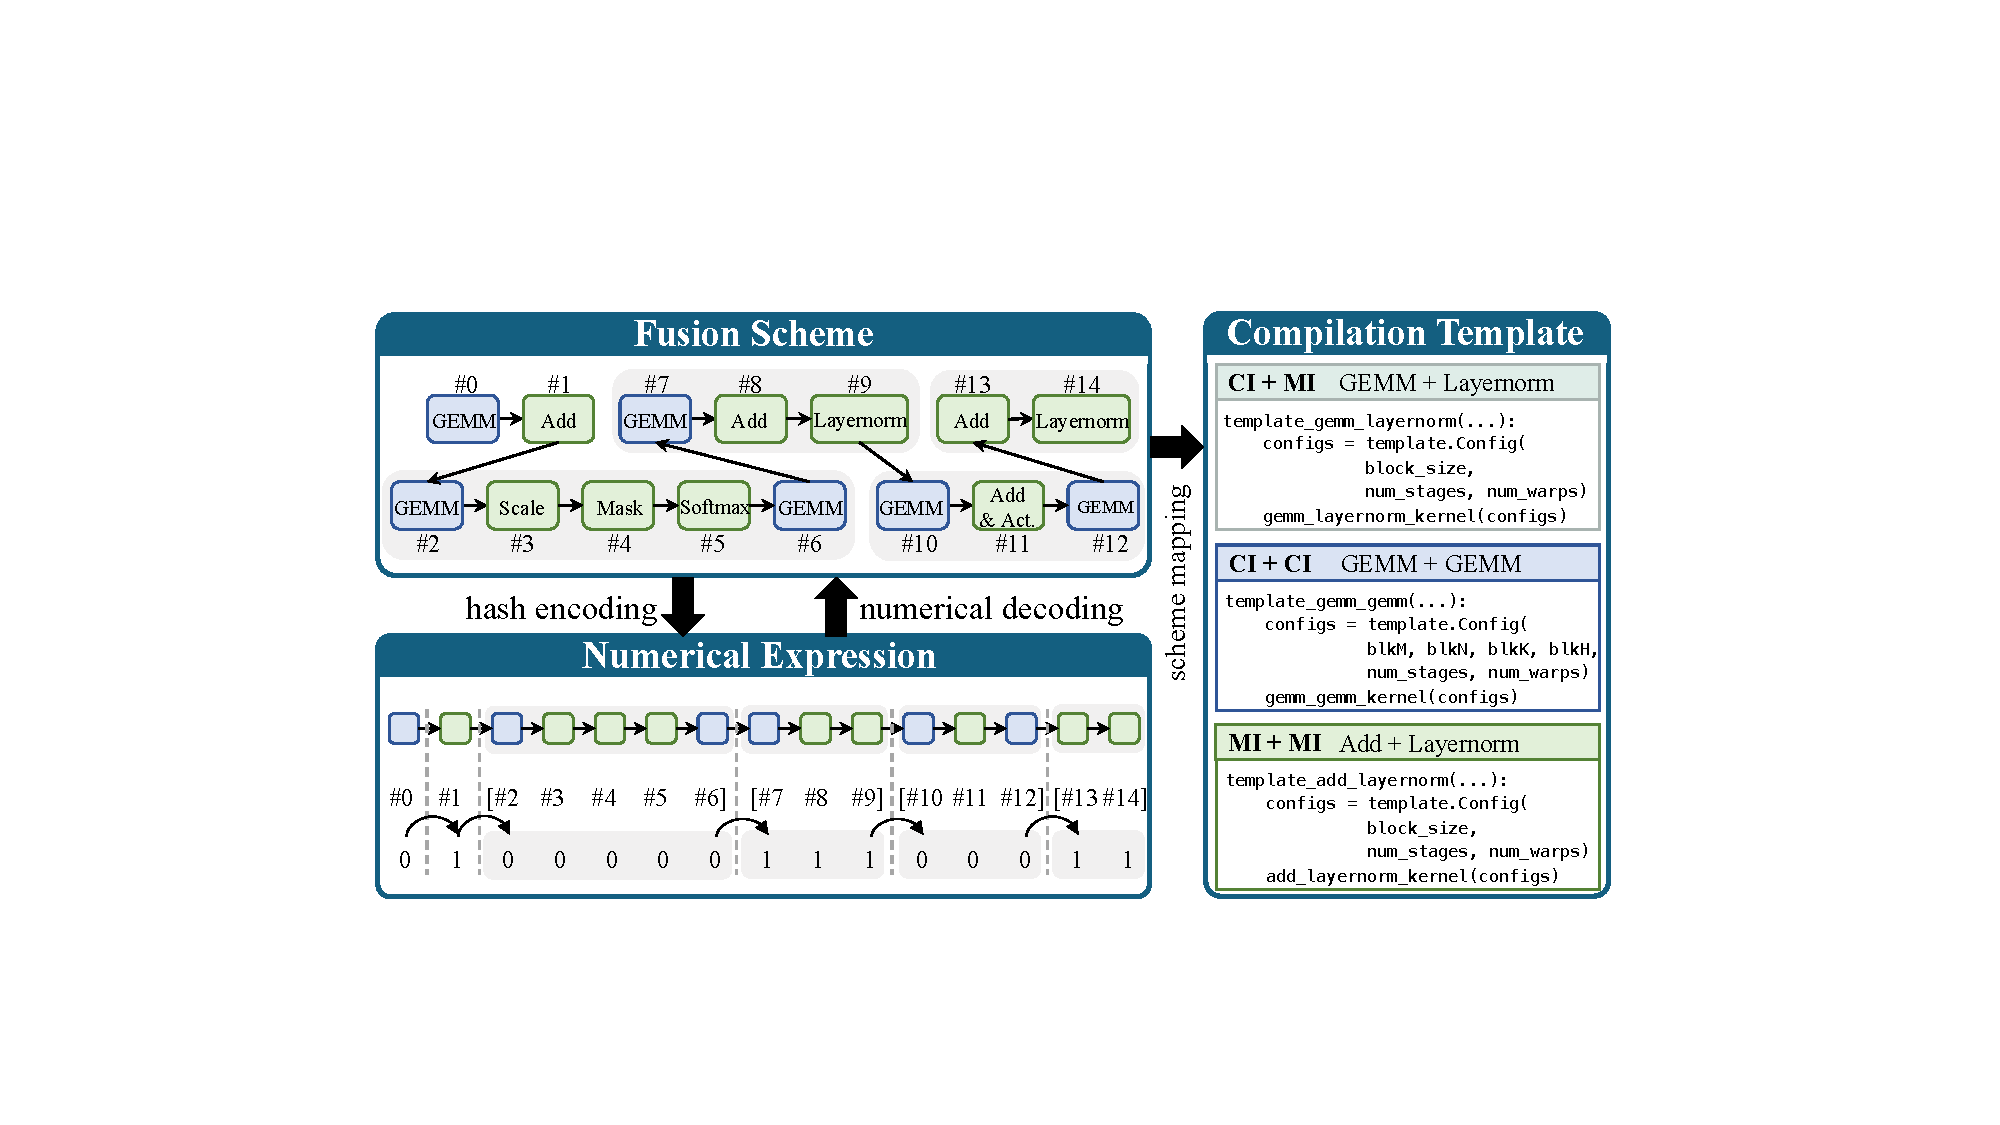
\includegraphics[width=\linewidth]{figures/4-method-encoding.pdf}
  %\vspace{-15pt}
  \caption{The workflow of fusion scheme converter.}
  \label{fig:4-method-encoding}
\end{figure}
% %\vspace{-5pt}

Figure~\ref{fig:4-method-encoding} shows the workflow of the fusion scheme converter in STOF. Take the forward propagation of BERT as an example, STOF traverses the computational graph constructed by the DL framework and extracts subgraphs that conform to the patterns of fusion schemes. Each subgraph is mapped to the target compilation template, which is carefully implemented to achieve optimal performance. Specifically, the templates decompose tensor operations into tiles to maximize data reuse, leverage warp-level primitives for efficient reductions, and apply multi-stage pipelining to overlap memory accesses and computation.
%by decomposing GEMM chains into hierarchical tiles to maximize data reuse, leveraging warp-level primitives for efficient reductions with minimal synchronization, configuring the number of warps (\texttt{warp\_num}) to control parallelism granularity, and applying multi-stage pipelining to overlap memory loads, computation, and write-back with tunable stages for balanced latency hiding and throughput.
Although we customize the compilation template according to the functionality of the fused operator, the graph mapping process is highly flexible. For instance, the template that computes a GEMM chain with CI+CI pattern can also incorporate simple MI operations, such as adding bias element by element (i.e., \texttt{Bias}). On the other hand, the compilation template hides the hardware execution details and only exposes key kernel parameters for performance tuning. For the GEMM chain, the sub-block sizes and the launch configuration (e.g., number of stages) constitute the search space, providing the possibility of further optimization targeting at a specified case.
%defined by the high-level language interface but retains partial hardware scheduling details. The compilation templates are
%, and expose parameters for subsequent tuning.


The fusion scheme is quantized by hash encoding, and the native operators are represented as arrays with a length equal to the number of operators according to the vertical fusion situation. 
In this way, hash encoding translates abstract fusion patterns into a quantifiable space, a process that establishes a bidirectional mapping consistent with the definition of ``hash''.
We assume that in addition to mapping MHA ([\#2-\#6]) to the fused kernel, the fusion scheme also specifies three other downstream fused operators including [\#7-\#9], [\#10-\#12], and [\#13,\#14]. 
%The above four fused operators are encoded as arrays composed of all 0s or all 1s, which is similar to the high-low voltage levels of the circuit. 
The numbers representing the operators in the subgraph are the same, which is similar to the high-low voltage levels of the circuit. 
For example, the numbers corresponding to the subgraph [\#7-\#9] are all 1. Besides, the different numbers of adjacent operators refer to the boundary of adjacent subgraphs. 
%Since the numbers corresponding to \#6 and \#10 are 0, the boundary operators of this subgraph are \#7 and \#9.
Note that the numbers are unrelated to the operator characteristics, they are introduced solely to facilitate the subsequent tuning process.
The numerical expression is usually in binary, but it can also be converted to hexadecimal format with a higher compression rate. Intuitively, this expression approach constructs a flexible search space that can represent any fusion scheme. On this basis, we propose a two-stage search mechanism to tune the running configuration during inference.
%fusion expansion and search space construction. 

\subsection{Search Space Exploration}
\label{sec:psc}

STOF deploys a search engine featuring scalable fusion boundaries and parameter-tuning capabilities. As depicted in Figure~\ref{fig:4-method-search}, 
the search engine first uses neural hashing and predefined rules to derive an initial fusion scheme. Then, the two-stage procedure is conducted to determine the boundaries of the fused operators and their kernel parameters.

%analyzes network information to derive an initial fusion scheme, then the search engine enters a two-stage tuning procedure. In the first stage, the boundaries of the fused operators are expanded according to specific rules until there is no additional benefit after fusion. In the second stage, parameter sampling is conducted on the determined fusion scheme, where the sampling ratio of the fused operators is adjusted based on the reward.

% SQX: 图的左侧，框里对号的内容改为computation graph，neural hashing和predefined rules
\begin{figure}[htbp]
  \centering
  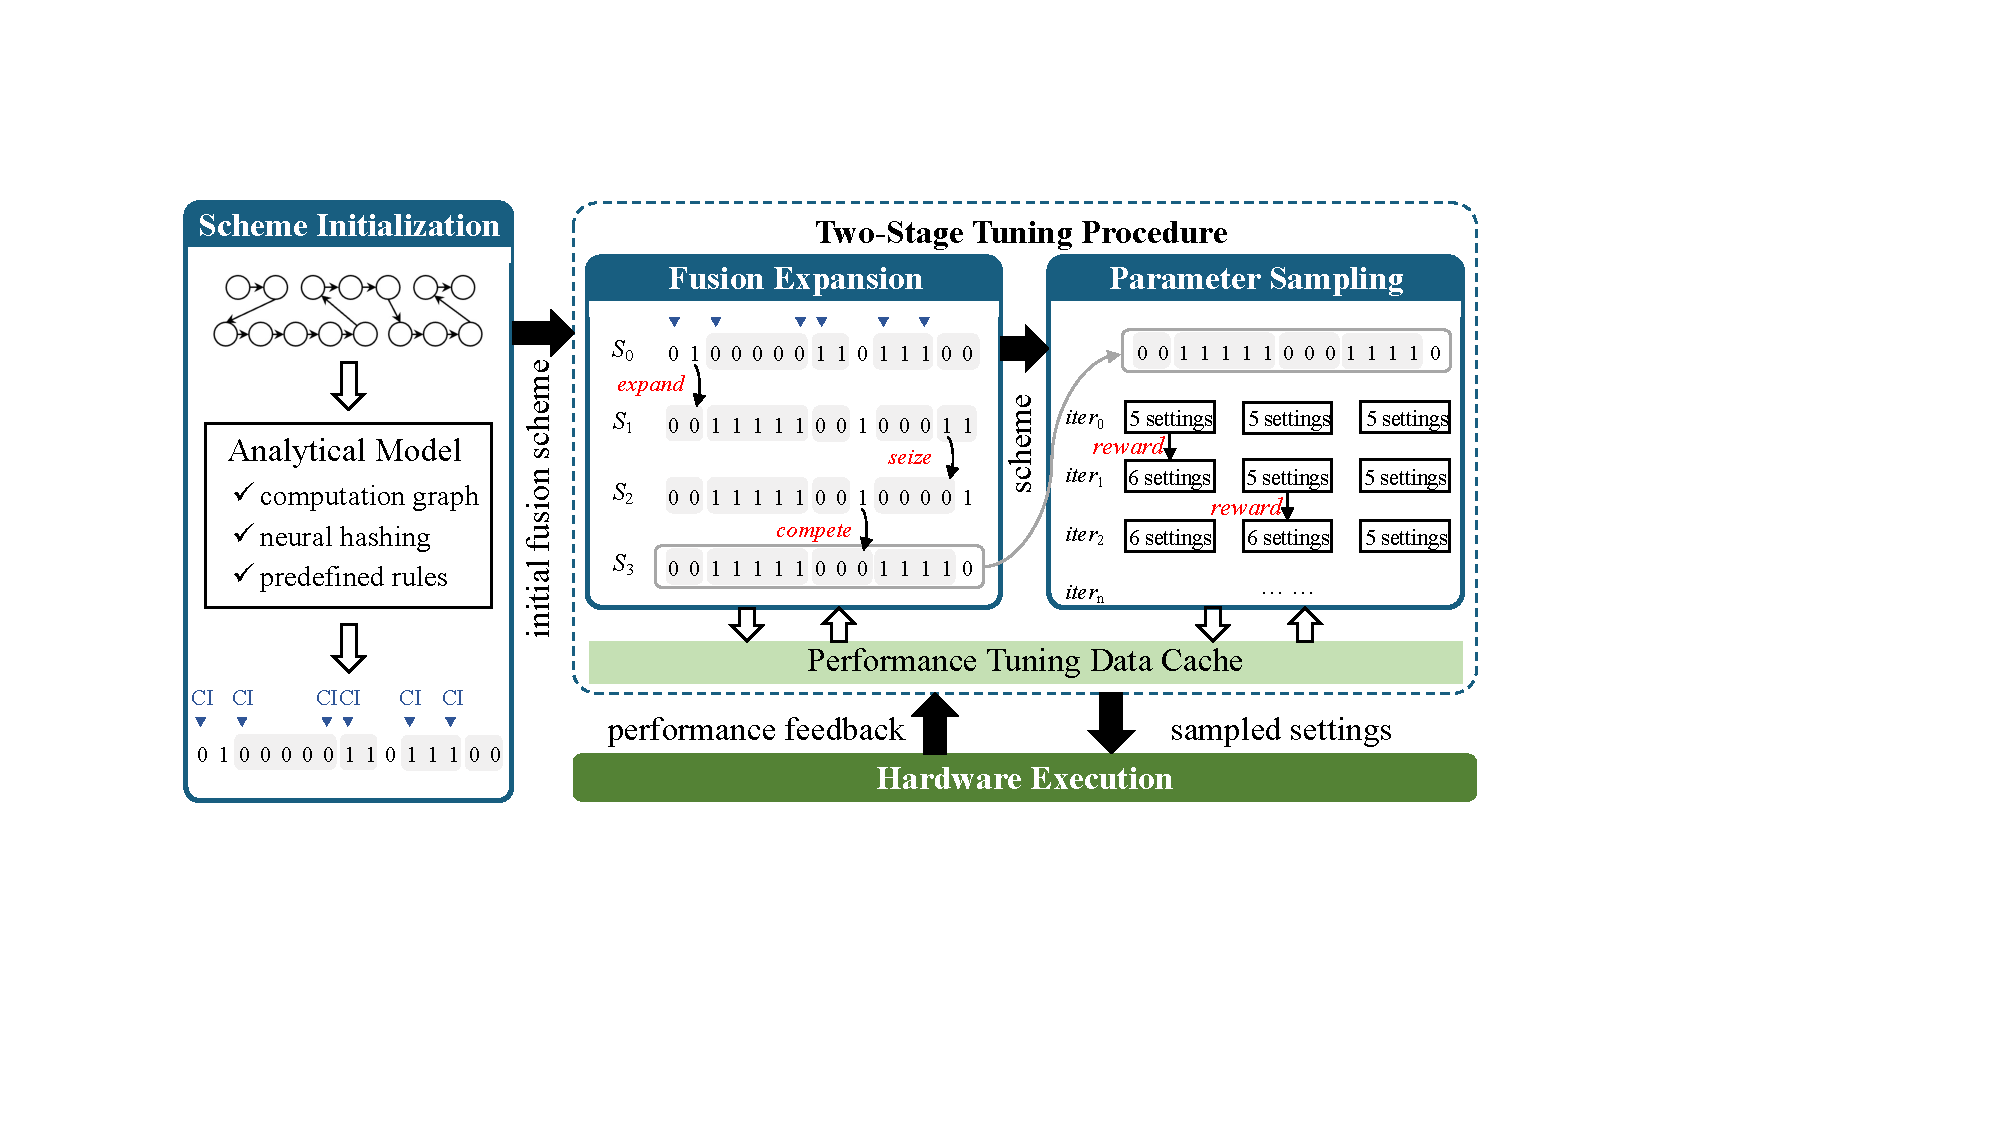
\includegraphics[width=\linewidth]{figures/4-method-search.pdf}
  %\vspace{-16pt}
  \caption{The workflow of hierarchical search engine.}
  \label{fig:4-method-search}
\end{figure}

\subsubsection{Fusion Scheme Initialization}
STOF leverages both pattern discovery and expert knowledge to derive the initial fusion scheme.
First, STOF adopts a convolutional subgraph analysis method \textit{neural hashing} to discover representative subgraphs that frequently appear during the inference, formalized as: $H(G) = \mathcal{F}_{\text{hash}}(\mathcal{F}_{\text{conv}}(G))$. Here, $G$ is the input computational graph structure; $\mathcal{F}_{\text{conv}}$ is a convolutional feature extractor that extracts local structural features from the graph $G$. $\mathcal{F}_{\text{hash}}$ is a hash mapper, which compresses and discretizes the extracted features into a unique hash fingerprint $H(G)$. By analyzing the frequency distribution of these fingerprints, STOF can rapidly detect classical subgraph structures across Transformer-based models. Second, STOF uses \textit{predefined rules} to extract potentially high-performance subgraphs from the identified subgraph structures to form the initial scheme.
For example, according to the conclusion in Section~\ref{sec:motivation}, the GEMM chain is preferentially fused into one segment under smaller batch sizes and sequence lengths.

% Specifically, STOF treats the computation graph as a sequence signal and uses convolutional layers to extract its local structural features offline.

%During the initialization process, instead of solely relying on predefined rules, STOF adopts an unconventional yet efficient Neural Hashing approach to discover representative subgraphs. Specifically, the computational graph is treated as a sequence signal, from which convolutional layers extract local structural features. 

%Although hash-based encoding may initially suffer from collisions, potentially leading to inaccurate matches, STOF progressively refines the hashing mechanism. This refinement is achieved through the joint optimization of the convolutional filters and the embedding space, enabling the model to minimize collisions and improve the precision of pattern discovery. 
%Consequently, neural hashing approach enhances the quality of the initial fusion scheme over time.
%not only accelerates the subgraph analysis process but also adaptively 

\subsubsection{Two-Stage Tuning Procedure}
In \textit{the first stage}, STOF tends to expand the boundaries of the segments until there is no additional benefit after fusion.
%STOF allows for the expansion of the fused operator, which is manifested as the extension of the segment boundaries. 
Since DL frameworks have implemented the fusion of common MI operators, we mark CI operators and adjust the fusion scheme around them for complementarity.
We have restricted that there are at most two CI operators in each segment, and classified the fusion rules into the following three categories.

\begin{itemize}
  \item \textit{expand}: merge existing individual or fused operators to form a new segment without disrupting the structure of other segments, such as the transition from $S_0$ to $S_1$.
  
  \item \textit{seize}: a segment with at least one CI operator preempts an operator from a segment consisting of only MI operators, such as the transition from $S_1$ to $S_2$.

  \item \textit{compete}: if two segments compete for an individual operator, the segment with only one CI operator will be extended first, such as the transition from $S_2$ to $S_3$.

\end{itemize}

Based on the above rules, we apply depth-first search (DFS) to gradually expand the fusion range. In this process, STOF randomly samples a fixed number of parameter settings of the pre-fusion and post-fusion operators, then takes the best setting to compare the performance. If there is a performance gain, STOF will keep the new fusion scheme, otherwise roll back. As long as the scheme has appeared and the performance under specific parameter settings is recorded in the cache, the same attempt will not be made later. 

In \textit{the second stage}, STOF conducts parameter sampling for the determined scheme. Specifically, we fix the total number of configurations during each iteration and retrieve performance data. In the first iteration, STOF ensures the number of sampled settings for each segment is the same. When the highest overall gain is achieved when tuning a segment, STOF rewards it by increasing the sampled settings in the next iteration. Similarly, STOF caches performance data to avoid repeated execution of the same parameter setting.


% shrpherding: 还需要添加一组 SPLAT 的实验；A100 / 4090 上
\begin{figure*}[htbp]
    \centering
    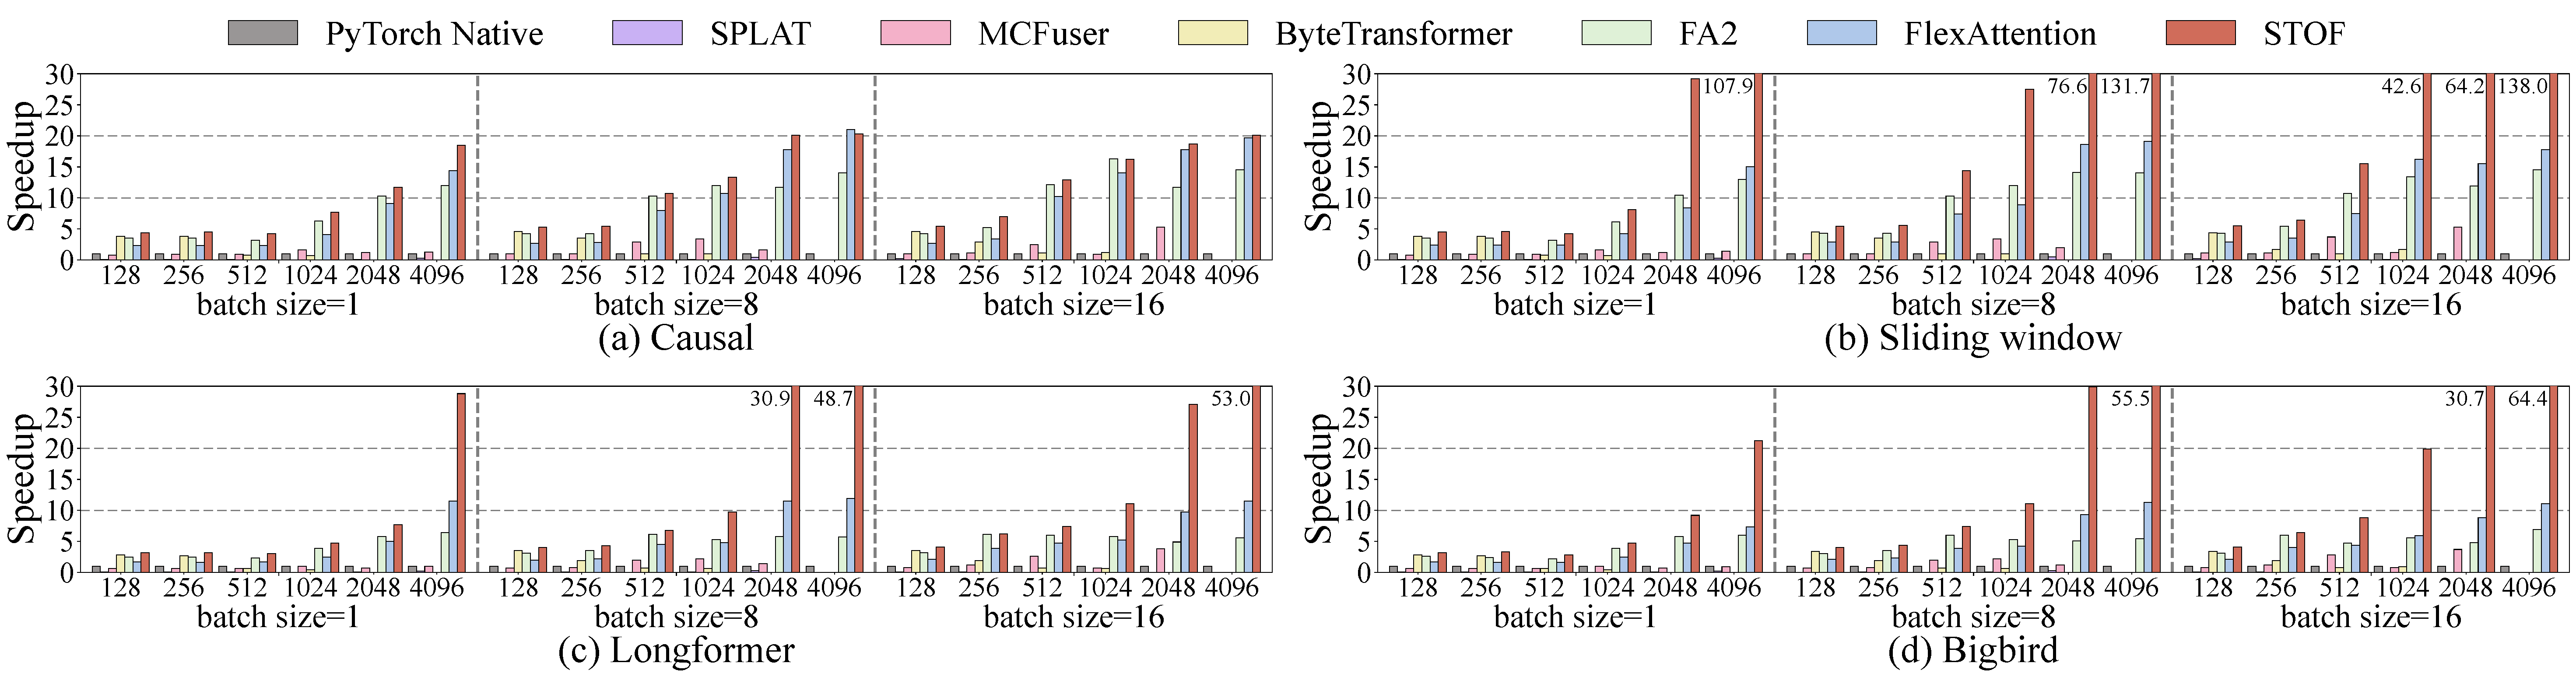
\includegraphics[width=\linewidth]{figures/5-eva-MHA-4090.pdf}        %4090的MHA于9/2/15:30更新,更新内容:将我们的kernel更换为block_m=64和block_n=64的分块
    \caption{The MHA performance of the methods normalized to that of PyTorch Native on NVIDIA RTX 4090 GPU.}
    \label{fig:MHA-evalaution-4090}
\end{figure*}

\begin{figure*}[htbp]
    \centering
    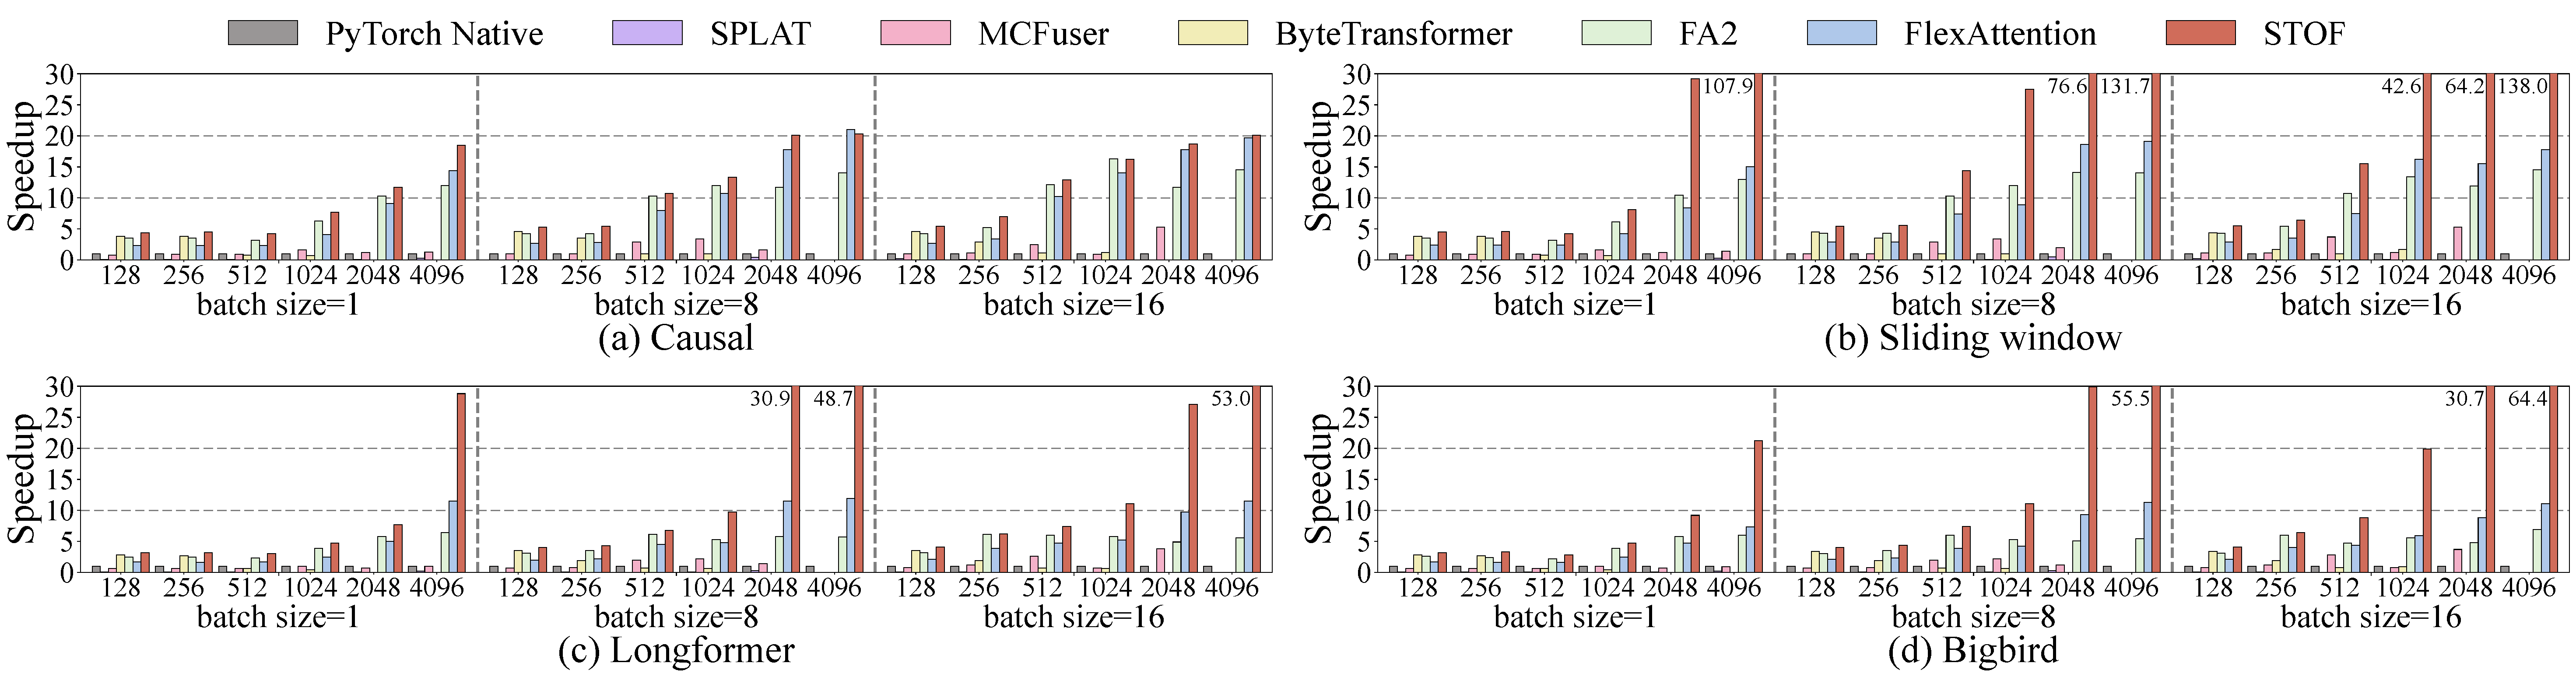
\includegraphics[width=\linewidth]{figures/5-eva-MHA-A100.pdf}         %A100的MHA于9/2/15:20更新,更新内容:将我们的kernel更换为block_m=64和block_n=64的分块
    \caption{The MHA performance of the methods normalized to that of PyTorch Native on NVIDIA A100 GPU.}
    \label{fig:MHA-evalaution-A100}
\end{figure*}


\subsection{Implementation Details}
\label{sec:impdetails}

We have implemented a system prototype of STOF based on PyTorch~\cite{ansel2024pytorch}, Triton~\cite{tillet2019triton} and TileLang~\cite{cheng2025pipethreader}, involving approximately 5,000 LOC of Python and 2,500 LOC of C/CUDA. 
%with \texttt{Jinja} used for the compilation template code rendering.ng. 
The block-wise kernel is developed based on FA2~\cite{dao2023flashattention2} with the CuTe structure, but introduces an efficient two-level storage format and corresponding optimizations.
%while introducing abstraction of sparse storage layout.
%\textcolor{blue}{with the CuTe structure to achieve efficient abstraction of sparse storage layout}. 
Subsequently, the customized MHA kernel is loaded into PyTorch through the \texttt{torch/cpp\_extension} interface, which encapsulates the kernel in the form of a native function.
When the MHA kernel is first called, it is just-in-time (JIT) compiled into a shared object file (\texttt{.so}) using the \texttt{ninja} tool, enabling dynamic linking at runtime without repeated compilation. 

% When the MHA kernel is first called, it is ahead-of-time (AOT) compiled into a shared object file (\texttt{.so}) using the \texttt{ninja} tool, enabling dynamic linking at runtime without repeated compilation. 

Regarding the operator fusion module, we find that the Triton- and TileLang-based compilation templates demonstrate performance variance under different fused operators, so we select the implementation that achieves superior performance in each case.
We enable the graph capture and replacement by manipulating objects of type \texttt{fx.GraphModule}. 
Since the overall implementation of STOF is
compatible with the \texttt{torch.compile} function, its related compilation optimizations can be reused to maximize performance.
%Since the non-intrusive implementation of STOF does not make any modifications to the PyTorch source code, it can be widely extended to other DNN scenarios or integrated into other DL backends.
%First, we insert the nodes that implement fusion, and then erase the invalid nodes. 

